% !TEX root = main.tex

\section{Analyzing a program with LLVM-MCA}


\begin{frame}{Preface}
Let's look at how MCA allows us to predict the performance of some code \alert{without running it}\\
\medskip
Two examples:
\begin{itemize}
\item Sum reduction
\item Matrix multiplication
\end{itemize}
\medskip
We will look at:
\begin{itemize}
\item C language source code
\item Assembly language produced by the compiler
\item Analysis of the assembly language made by LLVM-MCA
\end{itemize}
We will learn about how to use LLVM-MCA and how to interpret its results as we go.
\end{frame}


\input{15a-basics}
% !TEX root = main.tex

\subsection{Analyzing Resource Usage}


\begin{frame}{Hold on a sec, you cheater bastard!}
\begin{overprint}
\onslide<1>
Wait... weren't there \alert{some other instructions in the loop} apart from the sum!?
\onslide<2>
The results we looked at must have been completely wrong!
\end{overprint}
\begin{block}{Exhibit A}
\asminput[\tt\small]{listings/01_add_reduction_v1.s}
\end{block}
\end{frame}


\begin{frame}{I plead guilty!}
I surrender! You are right! I apologize! Let's annotate all the instructions in the loop!
\begin{block}{Remedial actions}
\asminput[\tt\small]{listings/01_add_reduction_v1b.s}
\end{block}
\end{frame}


\begin{frame}{I plead guilty!}
\begin{center}
Let's look at what's changed:
%
\begin{columns}

\column{0.45\textwidth}
\begin{block}{Before}
\asminput[\tt\small]{listings/01_add_reduction_v1_p01.txt}
\end{block}

\column{0.45\textwidth}
\begin{block}{After}
\asminput[\tt\small]{listings/01_add_reduction_v1b_p01.txt}
\end{block}

\end{columns}
\medskip
IPC, \emph{uOps Per Cycle} and \emph{Block RThroughput} are very different!\\
\end{center}
\end{frame}


\begin{frame}{I plead guilty!}
\begin{center}
\begin{block}{Bottleneck View}
\txtinput[\tt\fontsize{5.7pt}{6pt}\selectfont]{listings/01_add_reduction_v1b_p04.txt}
\end{block}
\medskip
\begin{overprint}
\onslide<1>
The bottleneck view unambiguously says that the biggest issue here is the update of the induction variable of the loop!
\onslide<2>
The perfect cure to this horrible disease is a classic and ever-lasting optimization: \alert{loop unrolling}!
\end{overprint}
\end{center}
\end{frame}


\begin{frame}{First Performance Improvement}
\begin{block}{Now we're talking!}
\asminput[\tt\small]{listings/01_add_reduction_v2.s}
\end{block}
\end{frame}


\begin{frame}{First Performance Improvement}
Let's run the old and the new modified program side by side to show to the world that I am the best programmer ever!\footnote{All experiments shown here were performed on a Intel Core i5-8259U CPU (Skylake microarchitecture) running at 2.30 GHz (peak 3.60 GHz).}
\begin{block}{Speedup Speedup Speedup}
\txtinput[\tt\small]{listings/01_add_reduction_v1_vs_v2_spdup.txt}
\end{block}
\pause
\alert{\centering WHAAAAAT!? The improvement is MINIMAL!\\}
\end{frame}


\begin{frame}{A closer look at the data}
\begin{block}{Timeline Comparison}
\asminput[\tt\fontsize{6.7pt}{7pt}\selectfont]{listings/01_add_reduction_v1_vs_v2_timeline.txt}
\end{block}
If we look at the timeline we can clearly see that LLVM-MCA \alert{correctly predicted} that the loop condition did not affect the sum operations, even without loop unrolling. 
\end{frame}


\begin{frame}{A closer look at the data}
\begin{columns}

\column{0.45\textwidth}
\begin{block}{Before}
\asminput[\tt\small]{listings/01_add_reduction_v1_p01.txt}
\end{block}

\column{0.45\textwidth}
\begin{block}{After}
\asminput[\tt\small]{listings/01_add_reduction_v1b_p01.txt}
\end{block}

\end{columns}
\medskip
In fact, the ratio between the total number of CPU cycles and the number of iterations was the same as well, regardless of whether we were including the loop condition.
\end{frame}


\begin{frame}{A closer look at the data}
\begin{columns}

\column{0.45\textwidth}
\begin{block}{Before}
\asminput[\tt\small]{listings/01_add_reduction_v1b_p01.txt}
\end{block}

\column{0.45\textwidth}
\begin{block}{After}
\asminput[\tt\small]{listings/01_add_reduction_v2_p01.txt}
\end{block}

\end{columns}
\medskip
The ratio between the total number of CPU cycles and the number of additions performed is the same  between the version with loop unrolling and the version without\\
\smallskip
{\footnotesize With loop unrolling each iteration performs 8 additions}
\end{frame}


\begin{frame}{The Resource Pressure View}
The reason why the loop condition computation can run in parallel with respect to the sum is that they require \alert{different CPU resources}.\\
\smallskip
We can see in detail the pressure on each resource from the \alert{Resource Pressure View}.
\bigskip
\begin{block}{Resource Pressure View}
\txtinput[\tt\fontsize{5.5pt}{6pt}\selectfont]{listings/01_add_reduction_v1b_p05.txt}
\end{block}
\end{frame}


\begin{frame}{The Resource Pressure View}
\begin{block}{Resource Pressure View}
\txtinput[\tt\fontsize{5.5pt}{6pt}\selectfont]{listings/01_add_reduction_v1b_p05.txt}
\end{block}
For each resource, this view shows the average number of resource cycles consumed at every iteration by the instructions.\\
\medskip
The concept of resources roughly corresponds to \alert{reservation stations} and the number and type of resources depends on the microarchitecture which is target of analysis.
\end{frame}


\begin{frame}{The Resource Pressure View}

\begin{columns}

\column{0.45\textwidth}
\begin{block}{Resource Pressure View: List of Resources}
\txtinput{listings/list-of-resources.txt}
\end{block}

\column{0.45\textwidth}

\begin{overprint}
\onslide<1>
\raggedright\bigskip
In our example, the CPU microarchitecture is \alert{Intel Skylake}.\\
We have \alert{7 \texttt{SKLPort} resources}.\footnotemark[1]
\begin{itemize}
\item \emph{SKL} is a contraction of \emph{SKyLake}
\item \emph{Port} means \emph{Reservation Station} in Intel's terminology
\end{itemize}
Each one of these resources serves different Functional Units.
\vfill
%
\onslide<2>
\begin{description}[\texttt{SKLPortM}]
\item[\texttt{SKLPort0}] Integer/float vector/scalar ALU, integer mul. and div., branch
\item[\texttt{SKLPort1}] Integer/float vector/scalar ALU
\item[\texttt{SKLPort2}] Load
\item[\texttt{SKLPort3}] Load
\item[\texttt{SKLPort4}] Store
\item[\texttt{SKLPort5}] Integer vector/scalar ALU
\item[\texttt{SKLPort6}] Integer scalar, branch
\item[\texttt{SKLPort7}] Store address
\end{description}
%
\onslide<3>
\raggedright\bigskip
The \texttt{SKLDivider} and \texttt{SKLFPDivider} resources are 
\alert{dummy resources}\\
\bigskip
They are used by the LLVM model to represent some complex
behavior that cannot be represented with a simulation based on simple pipelining.\\
\bigskip
Hardware-wise they don't exist.
\end{overprint}

\end{columns}

\footnotetext[1]{Additional information: \cite{fog-uarch}}

\end{frame}


\begin{frame}{A closer look at the data}
We can attempt to \alert{predict the execution time} using the total cycles / iteration count ratio.\\
\smallskip
Given that the actual program we are benchmarking executes $80\times10^{6}$ iterations:
\[
T_{exc} = \frac{N_{cycles}}{f_{ck}}
\]
\[
N_{cycles} = \frac{\textsf{Total Cycles}}{\textsf{Iterations}}80\times10^{6} \approx \frac{400}{100}80\times10^{6} = 320\times10^{6}
\]
\[
T_{exc} = \frac{320\times10^{6}}{3.6\times10^9 \si{\second}^{-1}} \approx \SI{0.088889}{\second}
\]
\end{frame}


\begin{frame}{A closer look at the data}
We measured an execution time of $0.10$ seconds, while LLVM-MCA estimates an execution time of $0.089$ seconds.
\bigskip
\begin{itemize}
\item The prediction by LLVM-MCA is close but not identical to the real value
\item The discrepancy can be attributed by the fact that LLVM-MCA does not simulate exactly every detail of the CPU, \emph{especially memory behavior}
	\begin{itemize}
	\item In fact, if we modify the program to always read from the same array element,
	the execution time drops to $\approx \SI{0.093175}{\second}$
	\end{itemize}
\end{itemize}
\end{frame}


\begin{frame}{What does this tell us?}
\large
\begin{enumerate}
\item We have to always pay attention to \alert{which} resources get used, not just how many are used
	\medskip
	\begin{itemize}
	\item Corollary: the loop condition usually does not interfere with the body of the loop
	\item We can mark just the body of the loop without too much worry!
	\end{itemize}
\bigskip
\item Traditional measurements of performance based on the instruction as the unit of work \emph{are deceptive and useless}
	\medskip
	\begin{itemize}
	\item Corollary: The performance numbers given by many CPU benchmarks are completely bogus and easy to manipulate
	\item The problem is that not every instruction performs the same amount of work!
	\end{itemize}
\end{enumerate}
\end{frame}


% !TEX root = main.tex

\subsection{Analyzing Data Dependencies}


\begin{frame}{Next optimization!}
Before we got sidetracked by the loop unrolling stuff, LLVM-MCA told us there was a \alert{data dependency} bottleneck
\begin{block}{Bottleneck View}
\txtinput[\tt\fontsize{5.7pt}{6pt}\selectfont]{listings/01_add_reduction_v1_p04.txt}
\end{block}
\end{frame}


\begin{frame}{Next optimization!}
The problem is that every sum we perform depends on the result of the previous one.
\bigskip
\begin{block}{Data Dependency Graph}
\begin{center}
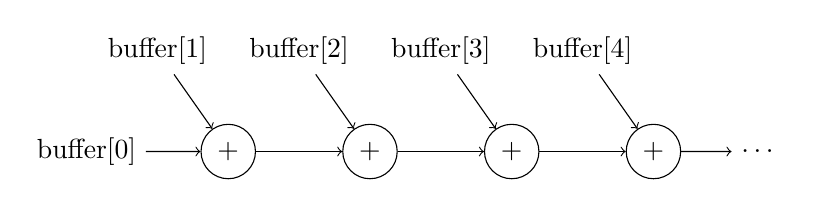
\begin{tikzpicture}[
		xscale=.9,yscale=0.64,
		inp/.style = {->},
		operation/.style = {circle, draw}
	]
	\node (b0) at (1,1) {buffer[0]};
	\node (b1) at (2,3) {buffer[1]};
	\node (b2) at (4,3) {buffer[2]};
	\node (b3) at (6,3) {buffer[3]};
	\node (b4) at (8,3) {buffer[4]};
	\node (sum0) [operation] at (3,1) {$+$};
	\node (sum1) [operation] at (5,1) {$+$};
	\node (sum2) [operation] at (7,1) {$+$};
	\node (sum3) [operation] at (9,1) {$+$};
	\node (dots) at (10.5,1) {\ldots};
	
	\path [inp] (b0) edge (sum0);
	\path [inp] (b1) edge (sum0);
	\path [inp] (b2) edge (sum1);
	\path [inp] (sum0) edge (sum1);
	\path [inp] (b3) edge (sum2);
	\path [inp] (sum1) edge (sum2);
	\path [inp] (b4) edge (sum3);
	\path [inp] (sum2) edge (sum3);
	\path [inp] (sum3) edge (dots);
\end{tikzpicture}

\medskip
\[
\textsf{result} = \left(\left(\left(\textsf{buffer[0]} + \textsf{buffer[1]}\right) + \textsf{buffer[2]}\right) + \textsf{buffer[3]}\right) + \ldots
\]
\end{center}
\end{block}
\end{frame}


\begin{frame}{Next optimization!}
If we exploit the associativity of addition, we can shorten the depth of our dependency chain!
\medskip
\begin{block}{Data Dependency Graph}
\small
\begin{center}
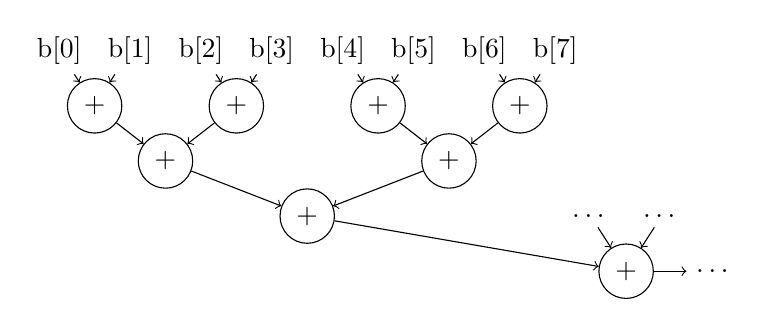
\begin{tikzpicture}[
		xscale=.45,yscale=0.7,
		inp/.style = {->},
		operation/.style = {circle, draw}
	]
	\node (b0) at ( 0,4) {b[0]};
	\node (b1) at ( 2,4) {b[1]};
	\node (b2) at ( 4,4) {b[2]};
	\node (b3) at ( 6,4) {b[3]};
	\node (b4) at ( 8,4) {b[4]};
	\node (b5) at (10,4) {b[5]};
	\node (b6) at (12,4) {b[6]};
	\node (b7) at (14,4) {b[7]};
	\node (sumL0I0) [operation] at (1,3) {$+$};
	\node (sumL0I1) [operation] at (5,3) {$+$};
	\node (sumL0I2) [operation] at (9,3) {$+$};
	\node (sumL0I3) [operation] at (13,3) {$+$};
	\node (sumL1I0) [operation] at (3,2) {$+$};
	\node (sumL1I1) [operation] at (11,2) {$+$};
	\node (sumL2I0) [operation] at (7,1) {$+$};
	\node (sumNext) [operation] at (16,0) {$+$};
	\node (dotsNextL1I0) at (15,1) {\ldots};
	\node (dotsNextL1I1) at (17,1) {\ldots};
	\node (dotsNextNext) at (18.5,0) {\ldots};
	
	\path [inp] (b0) edge (sumL0I0);
	\path [inp] (b1) edge (sumL0I0);
	\path [inp] (b2) edge (sumL0I1);
	\path [inp] (b3) edge (sumL0I1);
	\path [inp] (b4) edge (sumL0I2);
	\path [inp] (b5) edge (sumL0I2);
	\path [inp] (b6) edge (sumL0I3);
	\path [inp] (b7) edge (sumL0I3);
	\path [inp] (sumL0I0) edge (sumL1I0);
	\path [inp] (sumL0I1) edge (sumL1I0);
	\path [inp] (sumL0I2) edge (sumL1I1);
	\path [inp] (sumL0I3) edge (sumL1I1);
	\path [inp] (sumL1I0) edge (sumL2I0);
	\path [inp] (sumL1I1) edge (sumL2I0);
	\path [inp] (sumL2I0) edge (sumNext);
	\path [inp] (dotsNextL1I0) edge (sumNext);
	\path [inp] (dotsNextL1I1) edge (sumNext);
	\path [inp] (sumNext) edge (dotsNextNext);
\end{tikzpicture}

\end{center}
\[
\textsf{result} = \left(\left(\textsf{b[0]} + \textsf{b[1]}\right) + \left(\textsf{b[2]} + \textsf{b[3]}\right)\right) + \left(\left(\textsf{b[4]} + \textsf{b[5]}\right) + \left(\textsf{b[6]} + \textsf{b[7]}\right)\right) + \ldots
\]
\end{block}
\end{frame}


\begin{frame}{Next optimization!}
\begin{block}{Sum Reduction With Less Dependencies}
\cinput{listings/01_add_reduction_v3.c}
\end{block}
\end{frame}


\begin{frame}{Next optimization!}
\begin{columns}[onlytextwidth]

\column{0.7\textwidth}
\begin{block}{Sum Reduction With Less Dependencies}
\asminput[\tt\footnotesize]{listings/01_add_reduction_v3.s}
\end{block}

\column{0.25\textwidth}
\centering
LLVM is already helping the CPU scheduler by moving the access to \texttt{buffer[i+2]} before the access to \texttt{buffer[i+1]}!

\end{columns}
\end{frame}


\begin{frame}{What LLVM-MCA says...}
\begin{columns}

\column{0.45\textwidth}
\begin{block}{Before}
\asminput[\tt\small]{listings/01_add_reduction_v2_p01.txt}
\end{block}

\column{0.45\textwidth}
\begin{block}{After}
\asminput[\tt\small]{listings/01_add_reduction_v3_p01.txt}
\end{block}

\end{columns}
\medskip
The amount of work per iteration has stayed the same, and the cycle count is massively reduced!
\smallskip
From these figures, we expect the computation to complete in just $\approx\SI{0.01}{\second}$
instead than $\approx\SI{0.1}{\second}$!
\end{frame}


\begin{frame}{What the reality of facts says}
\begin{block}{Let's run it!}
\txtinput[\tt\small]{listings/01_add_reduction_v2_vs_v3_spdup.txt}
\end{block}
\medskip
\begin{description}[Good:]
\item[Good:] There is a huge improvement indeed!
\item[Bad:] The improvement is \alert{much less} than what we expected.
\end{description}
\end{frame}


\begin{frame}{The impact of memory accesses}
\begin{columns}

\column{0.55\textwidth}
\begin{block}{add\_reduction\_v3\_nocache.c}
\cinput[\tt\scriptsize]{listings/01_add_reduction_v3_nocache.c}
\end{block}
\begin{block}{Execution Time}
\txtinput[\tt\scriptsize]{listings/01_add_reduction_v3_nocache_spdup.txt}
\end{block}

\column{0.45\textwidth}
\begin{itemize}
\item Experiment: let's reduce the impact of memory accesses as much as possible
\item LLVM-MCA's analysis is the same even for the modified program
\item The real execution time now matches LLVM-MCA's prediction!
\end{itemize}

\end{columns}
\end{frame}


\begin{frame}{The impact of memory accesses}
\large
\begin{itemize}
\item Memory accesses are \alert{really slow}
\item Once the code is reasonably optimized, it will spend \alert{more time waiting for data to arrive} than performing actual calculations
\bigskip
\normalsize
\item This doesn't mean that, when it reaches that stage, the code cannot be optimized further.
\item Simply, any improvement from now on will be \alert{marginal}, especially for an algorithm like this one where there is not much we can do to improve memory access patterns.
\bigskip
\footnotesize
\item To solve the problem of memory access cost, some computer scientists have theorized computing systems where many small CPUs are embedded inside memory chips (\cite{MUTLU201928}).
\end{itemize}
\end{frame}


\begin{frame}{What can we do}
\begin{block}{Bottleneck View}
\txtinput[\tt\small]{listings/01_add_reduction_v3_p04.txt}
\end{block}
\begin{itemize}
\item We no longer have memory dependencies
\item Now it seems that we have excessive resource pressure
	\begin{itemize}
	\item \texttt{SKLPort2} and \texttt{SKLPort3} are used by \alert{load instructions}
	\item It seems we are issuing more loads than the CPU can perform 
	\end{itemize}
\end{itemize}
\end{frame}


\begin{frame}{What can we do}
\begin{itemize}
\item Let's scale back the ratio between memory accesses and add instructions a little bit...
\item Note that we are actually \alert{lengthening} the chain of data dependencies by doing this!
\end{itemize}

\begin{block}{Sum Reduction V3b}
\cinput{listings/01_add_reduction_v3b.c}
\end{block}
\end{frame}


\begin{frame}{Results}
\begin{block}{Sum Reduction V3b}
\txtinput{listings/01_add_reduction_v3_vs_v3b_spdup.txt}
\end{block}
\begin{itemize}
\item The tradeoff was worthwhile! We squeezed out some residual speedup from the code.
\end{itemize}
\end{frame}


\begin{frame}{In conclusion...}
We just made a piece of code \alert{worse} wrt. data dependencies... and there was a speedup!
\smallskip
\large
\begin{itemize}
\item You must always strike the right balance between different contrasting behaviors
	\begin{itemize}
	\item Data dependencies vs. resource usage
	\item Loop overhead vs. code cache and branch prediction
	\item Memory access patterns vs. algorithmic complexity
	\end{itemize}
\smallskip
\item You cannot reach the highest possible computation speed without machine-specific optimizations
	\begin{itemize}
	\item On a CPU architecture with more than 2 load ports, the situation is reversed and the code with 4 additions per cycle is now slower
	\end{itemize}
\end{itemize}
\end{frame}





% !TEX root = main.tex

\subsection{Recap}


\begin{frame}{Recap}
\begin{itemize}
\item LLVM-MCA analyzes the CPU performance of your machine code quite accurately
\item \alert{LLVM-MCA does not take into account the overhead of the memory hierarchy}
\item Analyze the views provided by LLVM-MCA carefully! Do not get tricked by irrelevant metrics.
\item Improve the code one bottleneck at a time
\item Perform large improvements first
\item When you find out that you are overfitting on your target machine, consider stopping
\medskip
\item {\footnotesize And it should go without saying, but...}\\
	{\normalsize\alert{Start with a good algorithm before you even consider using LLVM-MCA!}}
\end{itemize}
\end{frame}


\begin{frame}{Final Remarks}
\begin{itemize}
\item Most of the optimizations we made manually are applied automatically 
by LLVM when you use the \texttt{-ffast-math} flag
	\begin{itemize}
	\item This does not mean the techniques we saw are useless!
	\item It's just that our example was really simple
	\end{itemize}
\medskip
\item A further optimization that can be made is \alert{vectorization}
	\begin{itemize}
	\item Try it at home!
	\item Example code (alongside with all other examples shown here!):\\
				\url{https://github.com/danielecattaneo/LLVM-intro/tree/master/src/50-mca/example}
	\item We can lower the execution time to \SI{0.044824}{\second}
	\end{itemize}
\medskip
\item Not all CPUs are supported by LLVM-MCA!
	\begin{itemize}
	\item Check if yours is supported or not using \texttt{llc --version}!
	\end{itemize}
\end{itemize}
\end{frame}







